% !TEX program = xelatex
% AY2025 材料力学 解答例（同志社 生命医科学 医工学コース 院試）
% 問題・図は 01_exams/2025/tex を土台に、参考/ の粒度で解答を付した。
\documentclass[11pt,a4paper]{article}
\usepackage{../../00_common/preamble}
\usetikzlibrary{positioning,arrows.meta,calc,patterns,decorations.pathmorphing}

\title{材料力学 AY2025 解答例}
\author{}
\date{}

\begin{document}
\maketitle

\noindent\textbf{符号規約}：軸力・応力は引張りを正，圧縮を負とする．
〔I〕では下方への移動を正にとる．〔II〕では反力・たわみは荷重 $P$ の向き（下向き）を正，
たわみの基礎式は $EI\,\dfrac{d^2v}{dx^2}=M(x)$ を用い，曲げモーメントは下に凸を正とする．
断面二次モーメントは $I=\dfrac{\pi d^4}{64}$，断面二次極モーメントは $I_p=\dfrac{\pi d^4}{32}$．

%====================================================================
\section*{〔I〕}

図1のように, 剛体板が 2 本の棒\textcircled{1}（長さ $2L$, 断面積 $A$, 縦弾性係数 $E$）を介して天井から
釣り下がっており, 剛体板中央にある棒\textcircled{2}（長さ $L$, 断面積 $2A$, 縦弾性係数 $2E$）の上面に
荷重を負荷したところ, 上面が $\delta$ だけ下方に移動した. 各棒と剛体板の重さは無視できるとき,
次の問い (1)\,$\sim$\,(4) に答えよ.

\begin{center}
\begin{tikzpicture}[>=Latex,scale=0.85,baseline=(current bounding box.north)]
  \fill[pattern=north east lines] (-1.9,6) rectangle (1.9,6.35); \draw (-1.9,6) -- (1.9,6);
  \draw (-1.4,2) -- (-1.4,6); \draw (-1.3,2) -- (-1.3,6);
  \draw (1.3,2) -- (1.3,6); \draw (1.4,2) -- (1.4,6);
  \fill[gray!80] (-1.7,1.8) rectangle (1.7,2.0);
  \node[right] at (1.75,1.9) {剛体板};
  \fill[gray!55] (-0.5,2.0) rectangle (0.5,4.0); \draw (-0.5,2.0) rectangle (0.5,4.0);
  \draw[dashed] (-0.5,4.0) -- (2.8,4.0);
  \node at (-0.55,5.2) {棒\textcircled{1}}; \draw[->] (-0.7,5.0) -- (-1.25,4.6);
  \node at (0.9,5.2) {棒\textcircled{1}}; \draw[->] (1.05,5.0) -- (1.35,4.6);
  \draw[<->] (-1.75,2) -- (-1.75,6) node[midway,fill=white]{$2L$};
  \draw[<->] (-0.85,2) -- (-0.85,4) node[midway,fill=white]{$L$};
  \node at (0,-0.2) {荷重負荷前};
\end{tikzpicture}
\hspace{10mm}
\begin{tikzpicture}[>=Latex,scale=0.85,baseline=(current bounding box.north)]
  \fill[pattern=north east lines] (-1.9,6) rectangle (1.9,6.35); \draw (-1.9,6) -- (1.9,6);
  \draw (-1.4,1.5) -- (-1.4,6); \draw (-1.3,1.5) -- (-1.3,6);
  \draw (1.3,1.5) -- (1.3,6); \draw (1.4,1.5) -- (1.4,6);
  \fill[gray!80] (-1.7,1.3) rectangle (1.7,1.5);
  \node[right] at (1.75,1.4) {剛体板};
  \fill[gray!55] (-0.5,1.5) rectangle (0.5,3.5); \draw (-0.5,1.5) rectangle (0.5,3.5);
  \draw[dashed] (-2.8,4.0) -- (0.5,4.0);
  \draw[<->] (0.0,4.0) -- (0.0,3.5) node[midway,right]{$\delta$};
  \node at (0,-0.2) {荷重負荷後};
\end{tikzpicture}

\vspace{1mm}
図1
\end{center}

\subsection*{解答}

棒\textcircled{2}の上面に下向きの荷重 $P$ を負荷したものとする．荷重 $P$ は棒\textcircled{2}を通して剛体板に
伝わり，剛体板は 2 本の棒\textcircled{1}で天井から吊られている．よって棒\textcircled{1}は引張り，棒\textcircled{2}は
圧縮を受ける．棒\textcircled{1}の変位（伸び）を $\lambda_1$，棒\textcircled{2}の変位（縮み）を $\lambda_2$ とおく．

\medskip
\noindent\textbf{(1)}\quad 剛体板は水平のまま下方へ平行移動する（左右対称な 2 本の棒\textcircled{1}で吊られるため）．
棒\textcircled{1}が $\lambda_1$ 伸びると剛体板は $\lambda_1$ だけ下がる．さらに棒\textcircled{2}が $\lambda_2$ 縮むと，
その上面は剛体板に対してさらに $\lambda_2$ だけ下がる．したがって上面の下方移動 $\delta$ は両者の和である．
\[
  \ans{\;\delta = \lambda_1 + \lambda_2\;}
\]

\medskip
\noindent\textbf{(2)}\quad 鉛直方向のつり合いより，2 本の棒\textcircled{1}が分担する張力の和は荷重 $P$ に等しく，
左右対称だから 1 本あたり $P/2$．棒\textcircled{2}には圧縮力 $P$ が作用する．各棒の変位は
\[
  \lambda_1 = \frac{(P/2)(2L)}{A E} = \frac{PL}{AE},\qquad
  \lambda_2 = \frac{P\,L}{(2A)(2E)} = \frac{PL}{4AE}.
\]
これを (1) の関係式へ代入すると
\[
  \delta = \frac{PL}{AE} + \frac{PL}{4AE} = \frac{5PL}{4AE}.
\]
$P$ について解いて
\[
  \ans{\;P = \frac{4AE\,\delta}{5L}\;}
\]

\medskip
\noindent\textbf{(3)}\quad 棒\textcircled{1}は 1 本あたり張力 $P/2$，断面積 $A$，棒\textcircled{2}は圧縮力 $P$，断面積 $2A$ だから
\[
  \sigma_1 = \frac{P/2}{A} = \frac{P}{2A},\qquad
  \sigma_2 = \frac{P}{2A}.
\]
(2) の $P=\dfrac{4AE\delta}{5L}$ を代入すると
\[
  \ans{\;\sigma_1 = \sigma_2 = \frac{P}{2A} = \frac{2E\delta}{5L}\;}
\]
（$\sigma_1$ は引張り，$\sigma_2$ は圧縮で，大きさは等しい．）

\medskip
\noindent\textbf{(4)}\quad (2) の各式に $P=\dfrac{4AE\delta}{5L}$ を代入する．
\[
  \lambda_1 = \frac{PL}{AE} = \frac{4\delta}{5},\qquad
  \lambda_2 = \frac{PL}{4AE} = \frac{\delta}{5}.
\]
\[
  \ans{\;\lambda_1 = \frac{4}{5}\delta,\qquad \lambda_2 = \frac{1}{5}\delta\;}
\]
検算：$\lambda_1 + \lambda_2 = \dfrac{4\delta}{5}+\dfrac{\delta}{5} = \delta$ となり (1) の関係式を満たす ✓．
また $\sigma_1 = \dfrac{P}{2A} = \dfrac{E\lambda_1}{2L}$ に $\lambda_1=\tfrac{4}{5}\delta$ を入れると $\dfrac{2E\delta}{5L}$ で (3) と一致する ✓．

%====================================================================
\clearpage
\section*{〔II〕}

図2のように, 直角に折れ曲がった円形断面のはり（直径 $d$）の点 A が固定され, 点 C に下向きの
集中荷重 $P$ が作用する. 縦弾性係数を $E$, 横弾性係数を $G$ とし, 次の問い (1)\,$\sim$\,(4) に答えよ.
区間 AB（長さ $L$）は $x$ 軸方向，区間 BC（長さ $L/2$）は $y$ 軸方向にとり，荷重 $P$ は $z$ 軸負方向（下向き）とする．

\begin{center}
\begin{tikzpicture}[>=Latex]
  \fill[pattern=north east lines] (0.2,0.6) -- (0.2,3.0) -- (1.2,3.4) -- (1.2,1.0) -- cycle;
  \draw (0.2,0.6) -- (0.2,3.0) -- (1.2,3.4) -- (1.2,1.0) -- cycle;
  \draw[line width=11pt,gray!25,line cap=round] (0.9,2.4) -- (6.0,1.0);
  \draw[line width=11pt,gray!25,line cap=round] (6.0,1.0) -- (8.3,1.6);
  \draw[fill=gray!25] (8.3,1.6) ellipse (0.30 and 0.11);
  \draw[->] (0.9,2.4) -- (0.9,3.7) node[left]{$z$};
  \draw[->] (0.9,2.4) -- (2.0,2.95) node[above]{$y$};
  \draw[->] (6.0,1.0) -- (7.0,1.0) node[below]{$x$};
  \node[left] at (0.8,2.45) {A}; \node[below] at (6.0,0.7) {B}; \node[right] at (8.4,1.65) {C};
  \fill (2.3,2.25) circle (1.8pt); \node[above] at (2.3,2.3) {u};
  \draw[dashed] (2.3,1.95) ellipse (0.1 and 0.3);
  \node[below] at (2.3,1.75) {D};
  \draw[->,very thick] (8.3,2.7) -- (8.3,1.75); \node[right] at (8.35,2.5) {$P$};
  \draw[<->] (1.1,3.05) -- (6.0,1.65) node[midway,above,font=\scriptsize]{$L$};
  \draw[<->] (1.0,1.95) -- (2.3,1.6) node[midway,below,font=\scriptsize]{$L/4$};
  \draw[<->] (6.1,0.65) -- (8.3,1.25) node[midway,below,font=\scriptsize]{$L/2$};
  \begin{scope}[shift={(0.9,-1.6)}]
    \draw (0,0) circle (0.55);
    \draw[->] (0,-0.85) -- (0,0.95) node[right]{$z$};
    \draw[->] (-0.85,0) -- (0.95,0) node[above]{$y$};
    \fill (0,0.55) circle (1.8pt); \node[above left] at (0,0.55) {u};
    \node at (0,-1.25) {\underline{断面 D}};
  \end{scope}
\end{tikzpicture}

\vspace{1mm}
図2
\end{center}

\subsection*{解答}

点 A を原点とし，$\mathrm{A}(0,0,0)$，$\mathrm{B}(L,0,0)$，$\mathrm{C}\!\left(L,\tfrac{L}{2},0\right)$ とおく．
荷重は $\vec F=(0,0,-P)$．区間 AB の軸は $x$ 方向であるから，$x$ 軸まわりのモーメントが「ねじり」，
$y$ 軸まわりのモーメントが「曲げ」になる．

\medskip
\noindent\textbf{(1)}\quad 鉛直方向の力のつり合いより，固定端 A の支持力は荷重を支える上向きの力
$R_A = P$．点 A まわりのモーメントは，C の位置ベクトル $\vec r_{\mathrm C}=\left(L,\tfrac L2,0\right)$ を用いて
\[
  \vec M_A = -\,\vec r_{\mathrm C}\times\vec F
  = -\left(L,\tfrac L2,0\right)\times(0,0,-P)
  = \left(\tfrac{PL}{2},\,-PL,\,0\right).
\]
$y$ 軸成分が曲げモーメント，$x$ 軸成分がねじりトルクであるから，その大きさは
\[
  \ans{\;R_A = P\ (\text{上向き}),\qquad M_A = PL\ (\text{$y$ 軸まわり, 曲げ}),\qquad T_A = \frac{PL}{2}\ (\text{$x$ 軸まわり, ねじり})\;}
\]

\begin{center}
\begin{tikzpicture}[>=Latex,scale=0.9]
  \draw[line width=8pt,gray!25,line cap=round] (0,0) -- (4.5,0);
  \draw[line width=8pt,gray!25,line cap=round] (4.5,0) -- (6.5,0.9);
  \draw[pattern=north east lines] (-0.25,-0.8) rectangle (0,0.8); \draw (0,-0.8)--(0,0.8);
  \node[left] at (-0.3,0) {A}; \node[below] at (4.5,-0.3) {B}; \node[right] at (6.6,0.95) {C};
  \draw[->,very thick] (6.5,1.9) -- (6.5,1.0) node[midway,right]{$P$};
  \draw[->,very thick,blue] (0,-1.0) -- (0,0.2) node[below right]{$R_A=P$};
  \draw[->,very thick,red] (-0.2,0) arc (180:60:0.55) node[above]{$M_A=PL$};
  \draw[->,very thick,teal] (0.55,0.55) arc (110:-110:0.4) node[right]{$T_A=\tfrac{PL}{2}$};
\end{tikzpicture}
\end{center}

\medskip
\noindent\textbf{(2)}\quad 区間 AB（$0\le x\le L$）で断面位置 $x$ をとり，断面より先（C 側）の自由体を考える．
先端 C には下向きの荷重 $P$ のみが作用するから，断面に伝わるせん断力・曲げモーメント・ねじりトルクは
\[
  Q(x) = P\ (\text{一定}),\qquad
  M(x) = P\,(L-x),\qquad
  T(x) = P\cdot\frac{L}{2}\ (\text{一定}).
\]
端点での値は $M(0)=PL$（$=M_A$），$M(L)=0$（点 B で曲げ 0）．
\[
  \ans{\;Q(x)=P\quad(0\le x\le L),\qquad M(x)=P(L-x)\quad(M(0)=PL,\ M(L)=0)\;}
\]

\begin{center}
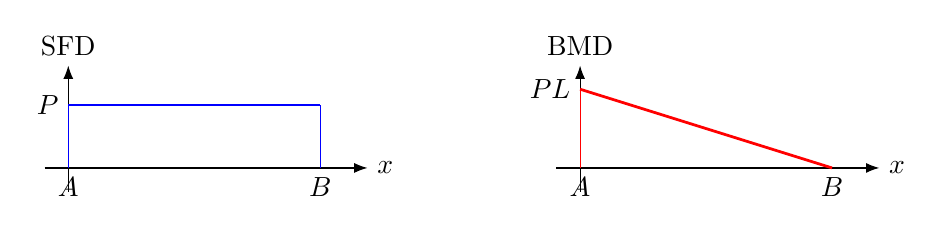
\begin{tikzpicture}[>=Latex,scale=1.0]
  \def\L{3.2}
  \begin{scope}
    \draw[->] (-0.3,0) -- (\L+0.6,0) node[right]{$x$};
    \draw[->] (0,-0.3) -- (0,1.3) node[above]{SFD};
    \draw[line width=1pt,blue] (0,0.8) -- (\L,0.8);
    \draw[blue] (0,0)--(0,0.8); \draw[blue] (\L,0)--(\L,0.8);
    \node[left] at (0,0.8) {$P$};
    \node[below] at (0,0) {$A$}; \node[below] at (\L,0) {$B$};
  \end{scope}
  \begin{scope}[xshift=6.5cm]
    \draw[->] (-0.3,0) -- (\L+0.6,0) node[right]{$x$};
    \draw[->] (0,-0.3) -- (0,1.3) node[above]{BMD};
    \draw[line width=1pt,red] (0,1.0) -- (\L,0);
    \draw[red] (0,0)--(0,1.0);
    \node[left] at (0,1.0) {$PL$};
    \node[below] at (0,0) {$A$}; \node[below] at (\L,0) {$B$};
  \end{scope}
\end{tikzpicture}
\end{center}

\medskip
\noindent\textbf{(3)}\quad 固定端 A から $L/4$ の断面 D では
\[
  M_D = P\!\left(L-\frac{L}{4}\right) = \frac{3PL}{4},\qquad
  T_D = \frac{PL}{2},\qquad Q_D = P.
\]
点 u は断面の最上点（$z=+d/2$）にある．\\
$x$ 方向応力（曲げ応力，$y$ 軸まわりの曲げ）は，$z=d/2$ で
\[
  \sigma_x = \frac{M_D\,(d/2)}{I} = \frac{(3PL/4)(d/2)}{I} = \frac{3PLd}{8I}
  \quad\left(=\frac{24PL}{\pi d^3}\right).
\]
$y$ 方向（軸に直交する方向）には垂直応力は生じないので $\sigma_y=0$．\\
せん断応力は，横せん断力 $Q$ による応力が断面最上端（極端繊維）で 0 となるため，ねじりによる
ねじりせん断応力のみが残り，その大きさは
\[
  \tau_{xy} = \frac{T_D\,(d/2)}{I_p} = \frac{(PL/2)(d/2)}{I_p} = \frac{PLd}{4I_p}
  \quad\left(=\frac{8PL}{\pi d^3}\right).
\]
\[
  \ans{\;\sigma_x = \frac{3PLd}{8I}=\frac{24PL}{\pi d^3},\qquad \sigma_y = 0,\qquad
       \tau_{xy} = \frac{PLd}{4I_p}=\frac{8PL}{\pi d^3}\;}
\]
検算：$I=\dfrac{\pi d^4}{64}$ より $\sigma_x=\dfrac{3PLd}{8}\cdot\dfrac{64}{\pi d^4}=\dfrac{24PL}{\pi d^3}$，
$I_p=\dfrac{\pi d^4}{32}$ より $\tau_{xy}=\dfrac{PLd}{4}\cdot\dfrac{32}{\pi d^4}=\dfrac{8PL}{\pi d^3}$ ✓．

\medskip
\noindent\textbf{(4)}\quad
\textbf{点 B のたわみ $\delta_B$}：区間 AB は固定端 A の片持ちはりで，内力の曲げモーメントは
$M(x)=P(L-x)$（先端 B に下向き荷重 $P$ を受ける片持ちと等価）．基礎式 $EI\,v''=M(x)$ を
$v(0)=0,\ v'(0)=0$ のもとで 2 回積分すると
\[
  EI\,v(x) = \frac{P}{2}Lx^2 - \frac{P}{6}x^3,\qquad
  EI\,v'(x) = PLx - \frac{P}{2}x^2 .
\]
よって点 B（$x=L$）で
\[
  \ans{\;\delta_B = \frac{PL^3}{3EI}\quad(\text{下向き})\;}
\]
また点 B での曲げによる傾き（$y$ 軸まわり）は $\theta_B = v'(L) = \dfrac{PL^2}{2EI}$．

\smallskip
\textbf{点 B のねじれ角 $\psi_B$}：区間 AB には一定のねじりトルク $T=\dfrac{PL}{2}$ が作用するから
\[
  \ans{\;\psi_B = \frac{T\,L}{G I_p} = \frac{PL^2}{2GI_p}\;}
\]

\smallskip
\textbf{点 C のたわみ $\delta_C$}：C の下方移動は次の 3 つの和である．
\begin{itemize}
  \item 区間 AB の曲げによる B の沈下 $\delta_B = \dfrac{PL^3}{3EI}$（C は B と同じ $z$ 変位を受ける）．
  \item 区間 AB のねじれ角 $\psi_B$ により，腕 BC（長さ $L/2$）の先端 C が $\psi_B\cdot\dfrac{L}{2}$ だけ沈下．
  \item 区間 BC 自体の曲げ（B を固定とみた長さ $L/2$ の片持ちに先端荷重 $P$）による先端たわみ
        $\dfrac{P(L/2)^3}{3EI}=\dfrac{PL^3}{24EI}$．
\end{itemize}
（区間 AB の曲げ傾き $\theta_B$ は $y$ 軸まわりの回転であり，C は B から $y$ 方向に離れているため
$z$ 変位には寄与しない．）したがって
\[
  \delta_C = \frac{PL^3}{3EI} + \psi_B\cdot\frac{L}{2} + \frac{PL^3}{24EI}
  = \frac{PL^3}{3EI} + \frac{PL^3}{4GI_p} + \frac{PL^3}{24EI}.
\]
$\dfrac{1}{3}+\dfrac{1}{24}=\dfrac{3}{8}$ より
\[
  \ans{\;\delta_C = \frac{3PL^3}{8EI} + \frac{PL^3}{4GI_p}\;}
\]
検算：剛性 $G\to\infty$（ねじれない）極限では $\delta_C\to\dfrac{3PL^3}{8EI}$ となり，
曲げのみの寄与（AB の $\tfrac{PL^3}{3EI}$ と BC の $\tfrac{PL^3}{24EI}$ の和）に一致する ✓．

\end{document}
